\documentclass[12pt]{article}

\usepackage[german]{babel}
\usepackage{amsmath}
\usepackage{amssymb} % to display symbols for real numbers, integers etc. Usage: \mathbb{R}
\usepackage{graphicx}
\usepackage{listings} % to display programming code
%\usepackage[ngerman]{babel}
\usepackage{color}
\usepackage{relsize} % to display scaled math symbols (big summation symbol etc.)
\usepackage{textcomp}

\DeclareGraphicsExtensions{.pdf,.jpeg,.png}
\definecolor{listinggray}{gray}{0.9}
\definecolor{lbcolor}{rgb}{0.9,0.9,0.9}
\lstset{ % to display programming code in nice colors
	backgroundcolor=\color{lbcolor},
	tabsize=4,
	rulecolor=,
	language=matlab,
		basicstyle=\scriptsize, %for extra small font size
        upquote=true,
        aboveskip={1.5\baselineskip},
        columns=fixed,
        showstringspaces=false,
        extendedchars=true,
        breaklines=true,
        prebreak = \raisebox{0ex}[0ex][0ex]{\ensuremath{\hookleftarrow}},
		frame=single, %draw frame
        showtabs=false,
        showspaces=false,
        showstringspaces=false,
        identifierstyle=\ttfamily,
        keywordstyle=\color[rgb]{0,0,1},
        commentstyle=\color[rgb]{0.133,0.545,0.133},
        stringstyle=\color[rgb]{0.627,0.126,0.941},
        numbers=left,
        stepnumber=1,
        firstnumber=1,
        numberfirstline=true,
        linewidth=14cm,
}

\title{Uebungsblatt 5\\ \glqq Mustererkennung\grqq}
\author{J. Cavojska, N. Lehmann, R. Toudic}
\date{08.06.2015}
\begin{document}
\maketitle
%\renewcommand{\contentsname}{Table of Contents}
\tableofcontents
\newpage

\section{Schnitte von zwei Gau\ss kurven}

\begin{align*}
f_1(x,\mu_1,\sigma_1) &= \frac{1}{\sqrt{2 \pi \sigma_1^2}} \cdot e^{-\frac{(x-\mu_1)^2}{2 \sigma_1^2}}\\
f_2(x,\mu_2,\sigma_2) &= \frac{1}{\sqrt{2 \pi \sigma_2^2}} \cdot e^{-\frac{(x-\mu_2)^2}{2 \sigma_2^2}}\\
\end{align*}
\underline{Eigenschaften von Dichtfunktionen $f_i$ f\"ur $\sigma_i > 0$ mit $i \in \mathbb{N}$}:
\begin{itemize}
\item $f_i$ ist achsensymmeterisch um $\mu_i$
\item $f_i$ hat zwei Wendepunkte: $\mu_i - \sigma_i$ und $\mu_i + \sigma_i$
\item $f_i$ hat genau ein Maximum bei $\mu_i$
\item $f_i$ ist stetig / f\"ur jede reelle Zahl definiert
\item $f_i(x,\mu_i,\sigma_i) > 0$
\end{itemize}
\underline{Eigenschaften von Dichtfunktionen $f_i$ f\"ur $\sigma_i = 0$ mit $i \in \mathbb{N}$}:
\begin{itemize}
\item $f_i$ ist nicht definiert
\item philosophische Betrachtung: $f_i$ ist eine Konstante!?
\end{itemize}
\underline{Eigenschaften von Dichtfunktionen $f_i$ f\"ur $\sigma_i < 0$ mit $i \in \mathbb{N}$}:
\begin{itemize}
\item $f_i$ ist nicht definiert in $\mathbb{R}$ (, aber in $\mathbb{C}$)
\end{itemize}
\newpage
\underline{Schnittpunkte von $f_1$ und $f_2$ bestimmen durch Gleichsetzung}:\\
\\
\textbf{Fall 1:} $\sigma = \sigma_1 = \sigma_2$\\
\begin{align*}
f_1(x,\mu_1,\sigma) &= f_2(x,\mu_2,\sigma) &\Leftrightarrow\\
\frac{1}{\sqrt{2 \pi \sigma^2}} \cdot e^{-\frac{(x-\mu_1)^2}{2\sigma^2}} &= \frac{1}{\sqrt{2 \pi \sigma^2}} \cdot e^{-\frac{(x-\mu_2)^2}{2 \sigma^2}} &\Leftrightarrow\\
e^{-\frac{(x-\mu_1)^2}{2\sigma^2}} &= e^{-\frac{(x-\mu_2)^2}{2 \sigma^2}} &\Leftrightarrow\\
log\left(e^{-\frac{(x-\mu_1)^2}{2\sigma^2}}\right) &= log\left(e^{-\frac{(x-\mu_2)^2}{2 \sigma^2}}\right) &\Leftrightarrow\\
-\frac{(x-\mu_1)^2}{2\sigma^2} \cdot log(e) &= -\frac{(x-\mu_2)^2}{2 \sigma^2} \cdot log(e) &\Leftrightarrow\\
-\frac{(x-\mu_1)^2}{2\sigma^2} &= -\frac{(x-\mu_2)^2}{2 \sigma^2} &\Leftrightarrow\\
(x-\mu_1)^2 &= (x-\mu_2)^2 &\Leftrightarrow\\
x^2 -2x\mu_1 + \mu_1^2 &= x^2 -2x\mu_2 + \mu_2^2 &\Leftrightarrow\\
2x\mu_1 - 2x\mu_2 + \mu_2^2 - \mu_1^2 &= 0 &\Leftrightarrow\\
x(2\mu_1 - 2\mu_2) + \mu_2^2 - \mu_1^2 &= 0 &\Leftrightarrow\\
x(2\mu_1 - 2\mu_2) &= \mu_1^2 - \mu_2^2 &\Leftrightarrow\\
x &= \dfrac{\mu_1^2 - \mu_2^2}{2\mu_1 - 2\mu_2} &\Leftrightarrow\\
x &= \dfrac{(\mu_1 + \mu_2) \cdot (\mu_1 - \mu_2)}{2(\mu_1 - \mu_2)} &\Leftrightarrow\\
x &= \dfrac{(\mu_1 + \mu_2)}{2}\\
\end{align*}
\textbf{Fall 2:} $\sigma_1 != \sigma_2$\\
\begin{align*}
f_1(x,\mu_1,\sigma_1) &= f_2(x,\mu_2,\sigma_2) &\Leftrightarrow\\
\frac{1}{\sqrt{2 \pi \sigma_1^2}} \cdot e^{-\frac{(x-\mu_1)^2}{2\sigma_1^2}} &= \frac{1}{\sqrt{2 \pi \sigma_2^2}} \cdot e^{-\frac{(x-\mu_2)^2}{2 \sigma_2^2}} &\Leftrightarrow\\
\frac{\sqrt{2 \pi \sigma_2^2}}{\sqrt{2 \pi \sigma_1^2}} \cdot e^{-\frac{(x-\mu_1)^2}{2\sigma_1^2}} &= e^{-\frac{(x-\mu_2)^2}{2 \sigma_2^2}} &\Leftrightarrow\\
\frac{\sqrt{2 \pi \sigma_2^2}}{\sqrt{2 \pi \sigma_1^2}} &= e^{-\frac{(x-\mu_2)^2}{2 \sigma_2^2} + {\frac{(x-\mu_1)^2}{2\sigma_1^2}}} &\Leftrightarrow\\
\frac{\sqrt{\sigma_2^2}}{\sqrt{\sigma_1^2}} &= e^{-\frac{(x-\mu_2)^2}{2 \sigma_2^2} + {\frac{(x-\mu_1)^2}{2\sigma_1^2}}} &\Leftrightarrow\\
ln \left(\frac{\sqrt{\sigma_2^2}}{\sqrt{\sigma_1^2}}\right) &= -\frac{(x-\mu_2)^2}{2 \sigma_2^2} + {\frac{(x-\mu_1)^2}{2\sigma_1^2}} &\Leftrightarrow\\
2 \sigma_2^2 \cdot ln \left(\frac{\sqrt{\sigma_2^2}}{\sqrt{\sigma_1^2}}\right) &= -(x-\mu_2)^2 + {\frac{2 \sigma_2^2 (x-\mu_1)^2}{2\sigma_1^2}} &\Leftrightarrow\\
2 \sigma_2^2 \cdot ln \left(\frac{\sqrt{\sigma_2^2}}{\sqrt{\sigma_1^2}}\right) &= -(x-\mu_2)^2 + {\frac{\sigma_2^2 (x-\mu_1)^2}{\sigma_1^2}} &\Leftrightarrow\\
2 \sigma_1^2 \sigma_2^2 \cdot ln \left(\frac{\sqrt{\sigma_2^2}}{\sqrt{\sigma_1^2}}\right) &= -\sigma_1^2(x-\mu_2)^2 + {\sigma_2^2 (x-\mu_1)^2} &\Leftrightarrow\\
2 \sigma_1^2 \sigma_2^2 \cdot ln \left(\frac{\sqrt{\sigma_2^2}}{\sqrt{\sigma_1^2}}\right) &= -\sigma_1^2(x^2 -2x\mu_2 + \mu_2^2) + {\sigma_2^2 (x-\mu_1)^2} &\Leftrightarrow\\
2 \sigma_1^2 \sigma_2^2 \cdot ln \left(\frac{\sqrt{\sigma_2^2}}{\sqrt{\sigma_1^2}}\right) &= -\sigma_1^2(x^2 -2x\mu_2 + \mu_2^2) + {\sigma_2^2 (x^2-2x\mu_1+\mu_1^2)} &\Leftrightarrow\\
2 \sigma_1^2 \sigma_2^2 \cdot ln \left(\frac{\sqrt{\sigma_2^2}}{\sqrt{\sigma_1^2}}\right) &= -\sigma_1^2x^2 +2x\mu_2\sigma_1^2 - \mu_2^2\sigma_1^2 + \sigma_2^2 (x^2-2x\mu_1+\mu_1^2) &\Leftrightarrow\\
2 \sigma_1^2 \sigma_2^2 \cdot ln \left(\frac{\sqrt{\sigma_2^2}}{\sqrt{\sigma_1^2}}\right) &= -\sigma_1^2x^2 +2x\mu_2\sigma_1^2 - \mu_2^2\sigma_1^2 + \sigma_2^2 x^2 -2x\mu_1\sigma_2^2 + \mu_1^2\sigma_2^2 &\Leftrightarrow\\
2 \sigma_1^2 \sigma_2^2 \cdot ln \left(\frac{\sqrt{\sigma_2^2}}{\sqrt{\sigma_1^2}}\right) + \mu_2^2\sigma_1^2 &= -\sigma_1^2x^2 +2x\mu_2\sigma_1^2 + \sigma_2^2 x^2 -2x\mu_1\sigma_2^2 + \mu_1^2\sigma_2^2 &\Leftrightarrow\\
2 \sigma_1^2 \sigma_2^2 \cdot ln \left(\frac{\sqrt{\sigma_2^2}}{\sqrt{\sigma_1^2}}\right) + \mu_2^2\sigma_1^2 - \mu_1^2\sigma_2^2&= -\sigma_1^2x^2 +2x\mu_2\sigma_1^2 + \sigma_2^2 x^2 -2x\mu_1\sigma_2^2 &\Leftrightarrow\\
2 \sigma_1^2 \sigma_2^2 \cdot ln \left(\frac{\sqrt{\sigma_2^2}}{\sqrt{\sigma_1^2}}\right) + \mu_2^2\sigma_1^2 - \mu_1^2\sigma_2^2&= x^2 (\sigma_2^2-\sigma_1^2) +2x\mu_2\sigma_1^2 -2x\mu_1\sigma_2^2 &\Leftrightarrow\\
\end{align*}
\newpage
\begin{align*}
2 \sigma_1^2 \sigma_2^2 \cdot ln \left(\frac{\sqrt{\sigma_2^2}}{\sqrt{\sigma_1^2}}\right) + \mu_2^2\sigma_1^2 - \mu_1^2\sigma_2^2&= x^2 (\sigma_2^2-\sigma_1^2) + 2x (\mu_2\sigma_1^2 - \mu_1\sigma_2^2) &\Leftrightarrow\\
\frac{2 \sigma_1^2 \sigma_2^2 \cdot ln \left(\frac{\sqrt{\sigma_2^2}}{\sqrt{\sigma_1^2}}\right) + \mu_2^2\sigma_1^2 - \mu_1^2\sigma_2^2}{\sigma_2^2-\sigma_1^2} &= x^2 + \frac{2x(\mu_2\sigma_1^2 - \mu_1\sigma_2^2)}{\sigma_2^2-\sigma_1^2}\\
\end{align*}
Ab hier gibt es zwei M\"oglichkeiten, die Gleichung zu l\"osen...
\begin{enumerate}
\item quadratische Erg\"anzung mit dem Term $\left(\frac{2(\mu_2\sigma_1^2 - \mu_1\sigma_2^2)}{\sigma_2^2-\sigma_1^2}\right)^2$ und umformen nach $x$
\item Term umformen und die P-Q-Formel verwenden
\end{enumerate}
Wir haben uns f\"ur die 2. Option entschieden:
\begin{align*}
x^2 + \frac{2x(\mu_2\sigma_1^2 - \mu_1\sigma_2^2)}{\sigma_2^2-\sigma_1^2} - \frac{2 \sigma_1^2 \sigma_2^2 \cdot ln \left(\frac{\sqrt{\sigma_2^2}}{\sqrt{\sigma_1^2}}\right) + \mu_2^2\sigma_1^2 - \mu_1^2\sigma_2^2}{\sigma_2^2-\sigma_1^2} &= 0 &\Leftrightarrow\\
x^2 + x \cdot \underbrace{\frac{2\mu_2\sigma_1^2 - 2\mu_1\sigma_2^2}{\sigma_2^2-\sigma_1^2}}_{P} - \underbrace{\frac{2 \sigma_1^2 \sigma_2^2 \cdot ln \left(\frac{\sigma_2}{\sigma_1}\right) + \mu_2^2\sigma_1^2 - \mu_1^2\sigma_2^2}{\sigma_2^2-\sigma_1^2}}_{Q} &= 0\\
\end{align*}
Nun k\"onnen wir die quadratische Gleichung mit der P-Q-Formel l\"osen.\\
\textit{Zur Erinnerung: Die P-Q-Formel lautet:} $x_{1/2} = -\frac{P}{2} \pm \sqrt{\left(\frac{P}{2}\right)^2 - Q}$.
\begin{align*}
x_1 &= \frac{\mu_1\sigma_2^2 - \mu_2\sigma_1^2}{\sigma_1^2-\sigma_2^2} + \sqrt{\left( \frac{\mu_2\sigma_1^2 - \mu_1\sigma_2^2}{\sigma_2^2-\sigma_1^2} \right)^2 + \frac{2 \sigma_1^2 \sigma_2^2 \cdot ln \left(\frac{\sigma_2}{\sigma_1}\right) + \mu_2^2\sigma_1^2 - \mu_1^2\sigma_2^2}{\sigma_2^2-\sigma_1^2}}\\
x_2 &= \frac{\mu_1\sigma_2^2 - \mu_2\sigma_1^2}{\sigma_1^2-\sigma_2^2} - \sqrt{\left( \frac{\mu_2\sigma_1^2 - \mu_1\sigma_2^2}{\sigma_2^2-\sigma_1^2} \right)^2 + \frac{2 \sigma_1^2 \sigma_2^2 \cdot ln \left(\frac{\sigma_2}{\sigma_1}\right) + \mu_2^2\sigma_1^2 - \mu_1^2\sigma_2^2}{\sigma_2^2-\sigma_1^2}}
\end{align*}
\newpage

\section{Klassifikation mit Fisher-Diskriminante}

Berechnete Werte fuer die Fisher-Diskriminante:\\
$w = [0.0019 -0.0019]$\\
$w0 = [13.6982  -13.8648]$\\
Details siehe Code:
\begin{lstlisting}[language=Matlab]
% Clean up
clear all
close all
clc

% Datenaufbreitung
Data         = load('fisher.txt');
Data0        = Data((Data(:,3)==0),:);
Data1        = Data((Data(:,3)==1),:);
Koordinaten  = Data(:,1:2);
Koordinaten0 = Data((Data(:,3)==0),1:2);
Koordinaten1 = Data((Data(:,3)==1),1:2);
Klassen      = Data(:,3);

% Aufgabe 2

% Grafik erstellen
figure('NumberTitle','off','Name','Aufgabe 2 - Bildpunkte');
    
X = Koordinaten(:,1);
Y = Koordinaten(:,2);
min_x = -250;
max_x =  250;
li = min_x:max_x;
    
% Punkte plotten
gscatter(X,Y,Klassen,'krb','+x',[],'off');
hold on

% Diskriminante erzeugen
FDK    = fitcdiscr(Koordinaten,Klassen);
Konst  = FDK.Coeffs(1,2).Const;
Linear = FDK.Coeffs(1,2).Linear;
fd = @(x1,x2) Linear(1)*x1 + Linear(2)*x2 + Konst;

% Fisher-Diskriminante plotten
Diskriminante = ezplot(fd, [min_x,max_x]);
Diskriminante.Color = 'b';
    
% Scatter within berechnen
mean1 = mean(Koordinaten0);
mean2 = mean(Koordinaten1);
S1 = 0;
for i = 1:size(Koordinaten0, 1)
    S1 = S1 + (Koordinaten0(i,:) - mean1)' * (Koordinaten0(i,:) - mean1);
end
S2 = 0;
for i = 1:size(Koordinaten1, 1)
	S2 = S2 + (Koordinaten1(i,:) - mean2)' * (Koordinaten1(i,:) - mean2);
end
S_w = S1 + S2;
  
% Vektor w berechnen:
w = inv(S_w) * (mean1 - mean2)';
w_norm = w / norm(w)
    
% Gerade durch den Vektor w legen und plotten
w_gerade_x = w_norm(1) * li;
w_gerade_y = w_norm(2) * li;
plot(w_gerade_y, w_gerade_x, 'g');    
    
% Daten auf Vektor w_norm projezieren
Koordinaten0_p = [];
for i = 1:size(Koordinaten0, 1)
    Koordinaten0_p = vertcat(Koordinaten0_p, Koordinaten0(i, :) * w_norm);
end
Koordinaten1_p = [];
for i = 1:size(Koordinaten1, 1)
    Koordinaten1_p = vertcat(Koordinaten1_p, Koordinaten1(i, :) * w_norm);
end
Koordinaten_p = vertcat(Koordinaten0_p, Koordinaten1_p);

% pdf der projizierten Daten aus Klasse 1 erzeugen
mean1_p = mean(Koordinaten0_p);
std1_p  = std(Koordinaten0_p);
pdf1_p  = pdf('Normal',li,mean1_p, std1_p);

% pdf der projizierten Daten aus Klasse 2 erzeugen
mean2_p = mean(Koordinaten1_p);
std2_p  = std(Koordinaten1_p);
pdf2_p  = pdf('Normal',li,mean2_p, std2_p);

% Schnittpunkt berechnen
[ispt_x,ispt_y] = intersections(li, pdf1_p, li, pdf2_p, 1);
    
% w0 berechnen und plotten
w0 = ispt_x * (w_norm')
plot(w0(1),w0(2),'m.','markersize',20);
    
% Titel, Bezeichner und Legende der Grafk
title('Aufgabe 2 - Plot');
xlabel('X-Koordinaten');
ylabel('Y-Koordinaten');
legend('1. Klasse','2. Klasse', 'Diskriminante', 'Gerade durch Vektor w', 'Punkt w_0')
axis([-50 300 -50 300])
\end{lstlisting}
Grafische Darstellung der Fisher-Diskriminante:\\
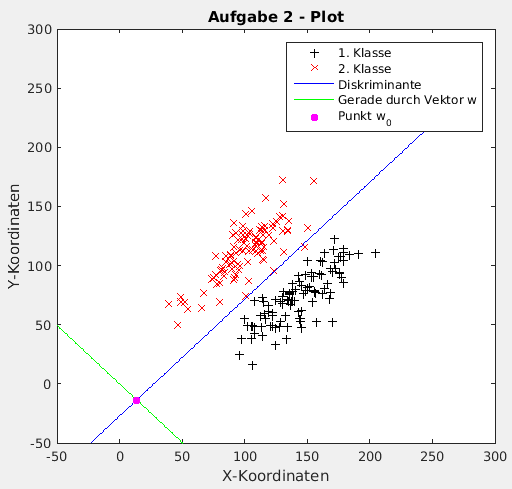
\includegraphics[width=10cm]{plot_fisher.png}\\
\newpage

\subsection{Mehr als 2 Klassen klassifizieren mit Bin\"arbaum}

Unser Algorithmus:

Sei K die Menge der Klassen, die wir voneinander trennen wollen.

\begin{enumerate}
\item F\"ur jede Klasse $K_i \in K$ wähle eine zuf\"allige Diskriminante $d_j$ als Wurzelknoten eines neuen Baums und f\"uhre die Punkte 2. und 3. f\"ur diese Klasse aus.
\item Entscheide, ob die Klasse $K_i$ links (-1) oder rechts (+1) von der Diskriminante $d_j$ liegt. Falls $K_i$ links von $d_j$ liegt, fuege zum $d_j$-Knoten ein linkes Kind hinzu, falls rechts, ein rechtes Kind. Markiere $d_j$ als bearbeitet.
\item W\"ahle eine Diskriminante $d_{j+1}$, die $d_j$ schneidet (und nicht bearbeitet ist) und gehe zu 2. Wenn diese nicht existiert, haben wir einen Pfad durch unseren Baum gefunden, der beschreibt, auf welcher Seite einer jeden Diskriminante unsere Klasse liegt.
\item Da die Reihenfolge, in der wir den Pfad zu einer Klasse durchlaufen, keine Rolle spielt (sondern nur das richtige Abbiegen), vereinigen wir alle Pfade in einen einzigen Bin\"arbaum (in 1. ist f\"ur jede Klasse ein eigener Bin\"arbaum entstanden).
\end{enumerate}
Jedes Blatt speichert eine Klasse $K_i$. Von dem Weg durch den Baum bis zu diesem Blatt ist f\"ur jede Diskriminante abzulesen, ob sie links von der Klasse $K_i$ (wir sind im Pfad in den linken Teilbaum reingegangen, um dieses Blatt zu erreichen) oder rechts davon (in den rechten Teilbaum rein) liegt.

\end{document}